%%
%% This is file `sample-lualatex.tex',
%% generated with the docstrip utility.
%%
%% The original source files were:
%%
%% samples.dtx  (with options: `sigconf')
%% 
%% IMPORTANT NOTICE:
%% 
%% For the copyright see the source file.
%% 
%% Any modified versions of this file must be renamed
%% with new filenames distinct from sample-lualatex.tex.
%% 
%% For distribution of the original source see the terms
%% for copying and modification in the file samples.dtx.
%% 
%% This generated file may be distributed as long as the
%% original source files, as listed above, are part of the
%% same distribution. (The sources need not necessarily be
%% in the same archive or directory.)
%%
%%
%% Commands for TeXCount
%TC:macro \cite [option:text,text]
%TC:macro \citep [option:text,text]
%TC:macro \citet [option:text,text]
%TC:envir table 0 1
%TC:envir table* 0 1
%TC:envir tabular [ignore] word
%TC:envir displaymath 0 word
%TC:envir math 0 word
%TC:envir comment 0 0
%%
%%
%% The first command in your LaTeX source must be the \documentclass command.
\documentclass[sigconf]{acmart}

\usepackage{listings}
\usepackage{hyphenat}
\usepackage{bm}
\usepackage{float}
\usepackage[T1]{fontenc}
\usepackage{hyperref,adjustbox}
\usepackage{graphicx}
\usepackage{pdfpages}
\usepackage[brazilian]{babel}
\usepackage{adjustbox}
\usepackage{multirow}
\usepackage{amssymb}
\usepackage{tabulary}
\usepackage{xcolor, soul}
\usepackage{pifont}% http://ctan.org/pkg/pifont
\newcommand{\cmark}{\ding{51}}%
\newcommand{\xmark}{\ding{55}}%
\usepackage{tikz}
\usepackage{natbib}
\usepackage[T1]{fontenc}
\usepackage{enumitem}

\usepackage{titlesec}


%%
%% \BibTeX command to typeset BibTeX logo in the docs
\AtBeginDocument{%
  \providecommand\BibTeX{{%
    \normalfont B\kern-0.5em{\scshape i\kern-0.25em b}\kern-0.8em\TeX}}}

%% Rights management information.  This information is sent to you
%% when you complete the rights form.  These commands have SAMPLE
%% values in them; it is your responsibility as an author to replace
%% the commands and values with those provided to you when you
%% complete the rights form.
\setcopyright{acmcopyright}
\copyrightyear{2018}
\acmYear{2018}
\acmDOI{10.1145/1122445.1122456}

%% These commands are for a PROCEEDINGS abstract or paper.
\acmConference[Woodstock '18]{Woodstock '18: ACM Symposium on Neural
  Gaze Detection}{June 03--05, 2018}{Woodstock, NY}
\acmBooktitle{Woodstock '18: ACM Symposium on Neural Gaze Detection,
  June 03--05, 2018, Woodstock, NY}
\acmPrice{15.00}
\acmISBN{978-1-4503-XXXX-X/18/06}


%%
%% Submission ID.
%% Use this when submitting an article to a sponsored event. You'll
%% receive a unique submission ID from the organizers
%% of the event, and this ID should be used as the parameter to this command.
%%\acmSubmissionID{123-A56-BU3}

%%
%% The majority of ACM publications use numbered citations and
%% references.  The command \citestyle{authoryear} switches to the
%% "author year" style.
%%
%% If you are preparing content for an event
%% sponsored by ACM SIGGRAPH, you must use the "author year" style of
%% citations and references.
%% Uncommenting
%% the next command will enable that style.
%%\citestyle{acmauthoryear}

%%
%% end of the preamble, start of the body of the document source.
\begin{document}

%%
%% The "title" command has an optional parameter,
%% allowing the author to define a "short title" to be used in page headers.
\title{Explorando contexto com métodos estado-da-arte para recomendação de vestimentas}

%%
%% The "author" command and its associated commands are used to define
%% the authors and their affiliations.
%% Of note is the shared affiliation of the first two authors, and the
%% "authornote" and "authornotemark" commands
%% used to denote shared contribution to the research.

\author{Heitor Werneck}
\affiliation{%
  \institution{Universidade Federal de São João del-Rei}
  %\city{São João del-Rei}
  \country{Brasil}
}
\email{werneck@aluno.ufsj.edu.br}

%\author{Leonardo Rocha}
%\affiliation{%
  %\institution{Universidade Federal de São João del-Rei}
  %%\city{São João del-Rei}
  %\country{Brasil}
%}
%\email{lcrocha@ufsj.edu.br}
%%
%% By default, the full list of authors will be used in the page
%% headers. Often, this list is too long, and will overlap
%% other information printed in the page headers. This command allows
%% the author to define a more concise list
%% of authors' names for this purpose.
\renewcommand{\shortauthors}{Werneck.}

%%
%% The abstract is a short summary of the work to be presented in the
%% article.
\begin{abstract}
A importância das vendas ‘online’ no espaço da moda de luxo cresce em um ritmo acelerado nos últimos anos, já que os consumidores das indústrias tradicionais agora esperam fácil acesso a uma rede mundial de marcas e varejistas. Para ter sucesso neste cenário, é necessário fornecer uma experiência de compra de moda sob medida, personalizada e confiável. Neste sentido, esse trabalho aborda um método que combina o contexto de um domínio com métodos de recomendação tradicionais, incorporando essas informações para atingir um nível maior de reconhecimento de padrões de interação para posterior inferência mais precisa das preferências dos usuários. O método proposto foi capaz de combinar quaisquer tipos de sistema de recomendação, particulamente neste trabalho combinamos um método de redes neurais de filtragem colaborativa com um método classico não-personalizado. O método apresentado mostrou ganhos significativos de até 80\% de MRR, 70\% de NDCG e 108\% de Hits.
\end{abstract}

%%
%% The code below is generated by the tool at http://dl.acm.org/ccs.cfm.
%% Please copy and paste the code instead of the example below.
%%

%\ccsdesc[500]{Computer systems organization~Embedded systems}
%\ccsdesc[300]{Computer systems organization~Redundancy}
%\ccsdesc{Computer systems organization~Robotics}
%\ccsdesc[100]{Networks~Network reliability}

%%
%% Keywords. The author(s) should pick words that accurately describe
%% the work being presented. Separate the keywords with commas.
\keywords{recommender systems, neural networks, cold-start, contextual recommender systems, stacking}

%% A "teaser" image appears between the author and affiliation
%% information and the body of the document, and typically spans the
%% page.

%%
%% This command processes the author and affiliation and title
%% information and builds the first part of the formatted document.
\maketitle

\section{Introdução}

Um crescimento explosivo de quantidade de informação na Internet criou um desafio de sobrecarga de informações que impede o acesso a itens de interesse. Esse fato aumentou a necessidade de sistemas de recomendação. Sistemas de recomendação são sistemas de filtragem de informações que lidam com o problema de sobrecarga de informações \cite{konstan2012recommender}, filtrando fragmentos de informações de uma grande quantidade de informações que é gerada dincamicamente por usuários utilizando um sistema de informação de acordo com seus interesses e prefêrencias sobre os itens do sistema. Um sistema de recomendação consegue prever se um determinado usuário preferiria um item ou não com base no histórico de consumo dos usuários.

Os sistemas de recomendação tem uma importância muito grande para grandes comércios, já que esse mesmo sistema consegue influenciar em quantos items são comprados \cite{jannach2019measuring}. Os ganhos de lucro são observados em diversos comércios, como, por exemplo: 35\% de aumento de vendas em um varejista de DVDs \cite{lee2014impact}; no eBay, \citeauthor{brovman2016optimizing} reportaram um aumento de 6\% em lucro na implantação de um novo método de recomendação comparado ao modelo linear que estava sendo utilizado; diversos exemplos de sucesso são encontrados na literatura \cite{jannach2019measuring}.

A importância das vendas ‘online’ no espaço da moda de luxo cresce em um ritmo acelerado nos últimos anos, já que os consumidores das indústrias tradicionais agora esperam fácil acesso a uma rede mundial de marcas e varejistas. Para ter sucesso neste cenário, é necessário fornecer uma experiência de compra de moda sob medida, personalizada e confiável. Os sistemas de recomendação desempenham um papel importante na jornada do usuário, permitindo que os clientes descubram produtos que atendem ao seu estilo, complementam suas escolhas ou os desafiam com novas ideias ousadas \cite{farfetchfashionrecommendationschallenge2021}.

Sistemas de recomendação de moda são tratados na literatura de diferentes prespectivas, como, por exemplo: \citeauthor{wang2014intelligent} integra temas de moda e percepção humana sobre formas corporais personalizadas e conhecimento de designers profissionais; \cite{dong2020interactive} apresenta um sistema de recomendação de roupas que utiliza informações do formato 3D do corpo. Geralmente a literatura sobre recomendação no domínio de moda é escassa em relação à literatura de outros domínios, porém recentemente há um crescimento de interesse sobre domínio \cite{he2016ups,frejlichowski2016finding,wakita2015fashion,kang2017visually,zeng2013intelligent}. Existem trabalhos que propõem diversas técnicas de filtragem colaborativa, porém estes trabalhos divergem em mínimos pontos, como, por exemplo no objetivo que varia muito de estudo para estudo, como, por exemplo o estudo de \citeauthor{hu2015collaborative} que foca na criação de conjuntos de roupa (recomendação de um conjunto de itens). Porém, geralmente há uma escassez de sistemas de recomendação que focam nesse domínio a partir de informações mais fundamentais da interação do usuário, as exceções são trabalhos como: \citeauthor{nguyen2014learning} que modela um método de learning to rank para recomendação personalizada de moda via feedback implicito (cliques, lista de desejos e compras), ainda é um método que pode ser generalizado para outros domínio e não há uma robusta avaliação quantitativa, comparando com métodos estado-da-arte, para comprovação de bons resultados.

Devido a complexidade da recomendação nesta área, o estudo de sistemas de recomendação tradicionais para a mesma é extremamente escasso, sendo o foco mais direcionado a exploração das carácteristicas que podem ser extraidas dos produtos (e.g., carácteristicas visuais das roupas) para futuras recomendações e criação de um conjunto de vestimenta.

Com base nisto, esse trabalho propõe uma experimentação de sistemas recomendação estado-da-arte em bases de dados reais de vestimentas assim como a proposta de um sistema de recomendação adequado para o domínio, sendo este um método de \textit{stacking} com redes neurais, que consegue fazer uso das informações de grande valor do domínio ao mesmo tempo que reaproveita abordagens gerais robustas.

\section{Conceitos Preliminares}

\subsection{Sistemas de recomendação contextuais}
Os sistemas de recomendação (SsR) tradicionais, como os baseados em filtragem colaborativa e baseado em conteúdo tendem a usar modelos de usuário bastante simples. Conforme observações adicionais são feitas sobre as preferências dos usuários, os modelos do usuário são atualizados e a preferência final inferida sobre o usuário é usada para gerar recomendações ou fazer previsões de avaliações dos mesmos. Esta abordagem ignora a noção de ações que possuem um contexto \cite{adomavicius2011context} e que os usuários interagem com o sistema em um contexto particular e as preferências relacionadas aos itens podem ser dependentes do contexto que o usuário está inserido.

Além destes SsR, SsR baseados em contexto utilizam vários tipos de informações contextuais para fazer recomendações. As informações contextuais podem ser \cite{haruna2017context}: espaciais, que são aqueles contextos que definem o estado geográfico ou ambiente dos usuários, ou itens; estáticos, são aqueles contextos que não mudam com o tempo e que afetam a recomendação, como idade, sexo, etc; temporais, diferentemente do contexto estático, são aqueles contextos que mudam temporamente e que são dinâmicos, como, por exemplo, o saldo do usuário na plataforma, relações sociais, etc.

Os SsR baseados em contexto são importantes para recomendação de vestimentas, pois, por exemplo, as roupas podem ter temporadas e podem ser recomendadas dependendo da estação do ano e seu pais. Tais informações contextuais podem melhorar a eficácia do processo de recomendação e nesse domínio é muitas vezes essencial. Informações contextuais são cada vez mais utilizadas assim como soluções para dominios específicos, utilizando suas informações de maneira específica, para melhorar o desempenho de um recomendador.

Os recomendadores que utilizam informações contextuais são cada vez mais utilizados para tratar o problema de cold-start \cite{zeng2016online,song2014online}, em cenários que essa informação está disponível esse é um recurso que pode possívelmente melhorar a recomendação de novos itens e usuários.

\subsection{Desafios em sistemas de recomendação}

Na tarefa de recomendação, os sistemas podem sofrer por diversos problemas nos dominios como~\cite{khusro2016recommender}: \textit{cold start problem}, onde um novo usuário ou item entra no sistema, ou também em uma definição mais leve esses mesmos elementos possuem pequeno histórico de interações; explicabilidade, que é geralmente encontrado a falta desse mesmo conceito em recomendadores baseados em redes neurais; \textit{grey sheep}, onde um usuário não concorda com nenhum outro grupo (métodos de filtragem colaborativa normalmente sofrem desse problema); esparsidade, onde os usuários normalmente interagem em um sistema com um amplo catálogo de items e a distinção entre interações sobre items de usuários torna a matriz de interações esparsa, o que pode levar a recomendações com menos acurácia.


\section{Trabalhos relacionados}

\citeauthor{bao2009stacking} propõe um método de \textit{stacking} para utilização em domínios mais tradicionais, com poucos atributos (criadas a partir dos dados de interação) e também se limitando a modelos simples com pouca capacidade de combinação de atributos em alto nível. \citeauthor{nguyen2014learning} propõe uma abordagem simples de recomendação para o domínio de moda no qual utiliza o preço do item, popularidade e o quão recente é o mesmo para auxiliar em recomendações, sendo uma estrátegia simples e muito pouco diversificada na exploração de atributos do domínio.

\citeauthor{kang2017visually} insere atributos visuais em sistemas de recomendação a partir de adaptações para melhorar a recomendação de itens de moda. \citeauthor{yin2019enhancing} propõem um método de aprendizagem de conhecimento de compatibilidade de moda que incorpora relações de compatibilidade visual, bem como informações de estilo. também propõe um método de recomendação de moda com estratégia de adaptação de domínio para aliviar a lacuna de distribuição entre os itens no domínio de destino e os itens de roupas externas compatíveis.

\citeauthor{cheng2016wide} propõe uma \textit{framework} para treinar em conjunto redes neurais feed-forward com embeddings e um modelo linear com transformações de atributos, apesar disso não há nenhuma discussão sobre a utilização de outros modelos de recomendação como entrada para o modelo. Outros trabalhos exploram a tarefa de recomendação de forma genérica, porém sem a utilização de informações adicionais além das interações \cite{he2020lightgcn,he2017neural,wu2021self}. Com isto, estes modelos sofrem de problemas em domínios no qual o contexto é muito importante, no entanto eles ainda descrevem uma parte importante da modelagem da interação entre usuário e item e novos modos de reaproveitamento dos métodos pre-existentes podem ser investigados.

No geral as abordagens da literatura estão preocupadas com desafios específicos na seleção de vestuário e não abordam uma avaliação com métodos estado-da-arte recentes de sistemas de recomendação tradicional. Além disso as abordagens genéricas que integram informações de contexto são complexas para o ajuste de hiper-parâmetros e não discutem o uso de sistemas pre-existentes para agregação de informação. Com isso este trabalho propõe preencher algumas lacunas, como:

\begin{enumerate}
  \item Uma avaliação de múltiplos sistemas de recomendação competitivos no domínio de recomendação de vestimentas;
  \item Uma abordagem mais adequada para o domínio de vestimentas, explorando informações do contexto junto com um método estado-da-arte em sistemas de recomendação;
  \item Demonstrar a importância do contexto na tarefa de recomendação de vestimentas;
  \item Melhorar as recomendações para diferentes tipos de usuários do sistema atráves do contexto.
\end{enumerate}


\section{Bases de Dados}

Para a experimentação foi coletado duas bases de dados que contém avaliações de usuários sobre produtos da Amazon, estas duas bases contém dados sobre a interação (i.e., timestamp da interação) e sobre o item (i.e., cor, tamanho, etc.).

\textbf{Amazon Fashion}. É uma base de dados de avaliações de usuários sobre itens na seção de moda da Amazon.

\textbf{Amazon Clothing}. É uma base de dados de avaliações de usuários sobre itens na seção de vestimentas (e.g., roupas, sapatos e joias),  da Amazon. Para a utilização da Amazon Clothing, devido ao grande número de interações, foi feito uma amostragem inicial aleatória de 100,000 usuários, com isso foi possível a sua utilização.

Essas duas bases de dados, sem nenhum tratamento especial possuem uma grande parcela de usuários com poucas interações, isto, para a avaliação de sistemas de recomendação baseados em filtragem colaborativa não é efetivo para uma análise quantitativa dos mesmos \cite{he2017neural}. Para uma avaliação mais diversa as duas bases passam por um processo de filtragem, onde somente usuários com menos que \textbf{n} interações são removidos da base de dados. Para a avaliação de dois importantes cenários de recomendação será utilizado $n=5$ para avaliar a base de dados com usuários com pouco e muito conhecimento, e $n=10$ para avaliação de usuários que contém um número razoável de interações (i.e., conhecimento para o sistema). Além disso, para simplificação da aplicação dos métodos e avaliação, as avaliações nessas bases de dados sobre o itens, que são valores de 1 a 5 são transformados em 1 caso sejam $\geq 4$ ou 0 caso contrário.

A Tabela \ref{tbl:dadosbases} apresenta as principais medidas estatisticas sobre as bases criadas.

\begin{table*}[ht]
  %\tiny
  \begin{tabular}{ccccc}
    Base de dados          & \#Usuários & \#Itens & \#Interações & Esparsidade\\\hline
    Amazon Fashion (n=5)   & 2056       & 7433    & 13452        & 99.91\%\\\hline
    Amazon Fashion (n=10)  & 128        & 1382    & 1654         & 99.06\%\\\hline
    Amazon Clothing (n=5)  & 7528       & 51029   & 70172        & 99.98\%\\\hline
    Amazon Clothing (n=10) & 2152       & 28338   & 36011        & 99.94\%\\\hline
\end{tabular}
\caption{Dados estátisticos das bases de dados.}
\label{tbl:dadosbases}
\end{table*}

\section{Explorando contexto com recomendadores estado-da-arte}

O método proposto consiste na combinação do contexto da interação (i.e., dia da interação, semana da interação, etc), com o contexto dos itens (e.g., material, cor, tamanho, preço, etc) e o contexto dos usuários (i.e., número de interações, número de itens consumidos) com métodos estado-da-arte tradicionais como pode ser visto na figura \ref{fig:model}. A abordagem irá fazer um \textit{stacking} de sistemas de recomendação, combinando suas predições com meta-dados que possibilitaram a exploração da modelagem pré-existente da interação usuário-item (atráves dos métodos já existentes, por exemplo: LightGCN) com um contexto que pode ser utilizado para reconhecer novos padrões de interação usuário-item. As redes neurais são abordagens comuns adotadas para soluções de sistemas de recomendação, modelos baseados em redes neurais possuem a capacidade de fazer combinação de atributos em multiplos níveis, com isso sendo capazes de solucionarem problemas complexos que as médidas alvo se exibem na combinação em alto nível de multiplos atributos. Combinando-os com modelos já existentes há a possibilidade de poupar esforços na modelagem da interação mais primitiva (no qual nenhum contexto é considerado) e direcionar mais esforços ao tratamento e preprocessamento dos daoos.

\begin{figure*}[ht]
    \centering
    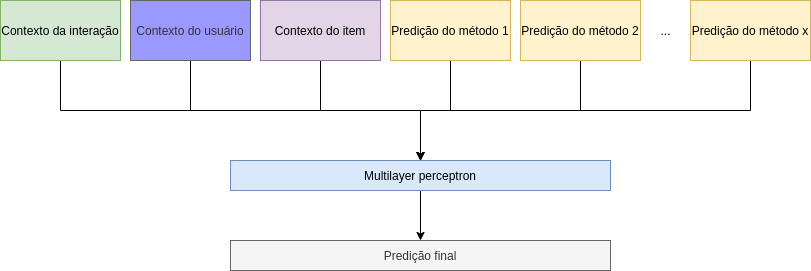
\includegraphics[width=0.75\textwidth]{./imgs/predictiondiagramdatamining.png}
    \caption{O framework de stacking proposto.}
    \label{fig:model}
\end{figure*}

A abordagem mais inicial e simples para combinar multiplas caracteristicas seria a utilização da multilayer perceptron (MLP) que é uma classe de rede neural artificial feedforward. Um MLP consiste de no mínimo três camadas de nós: uma camada de entrada, uma camada oculta e uma camada de saída. A partir da variação da arquitetura de uma MLP os resultados podem mudar bruscamente, uma arquitetura é altamente dependente do problema, sendo passivel de mudança brusca dependendo do problema a ser tratado. 

O MLP irá ter como entrada os seguintes atributos: predições dos modelos de recomendação (e.g., SVD, SVD++, etc); dados sobre o usuário; dados sobre a interação; dados sobre o item.

Para a utilização dos contextos mais adequadamente com a MLP será feito um preprocessamento inicial nos dados. Este preprocessamento irá transformar os atributos categóricos em vetores de atributos booleanos (one-hot encoding). Também em atributos onde um amplo número de categorias existem, somente as 100 mais populares são mantidas para evitar o problema da dimensionalidade nas recomendações. Também dois atributos relacionados ao usuário são utilizados a partir dos dados existentes para auxiliar na predição, sendo o número de interações e número de itens ''consumidos''. Outra estrátegia adotada para melhorar o aprendizado da rede foi aplicar a normalização z-score nas pontuações dadas pelos métodos.

Também para a adaptação adequada da rede ao problema será feito um método de busca de hiper-parâmetros atráves de 5-fold cross validation variando a estrutura da rede neural.

\section{Metodologia de avaliação}

A política de avaliação para medir a qualidade dos métodos na tarefa de recomendação adotada foi a avaliação \textit{leave-one-out}, sendo muito presente na literatura de sistemas recomendação \cite{he2017neural,rendle2012bpr}. Nesta metodologia de avaliação para cada usuário sua última interação (em ordem temporal) é inserida no conjunto de teste e os dados restantes são utilizados como treinamento. 

Além disso, devido ao custo elevado de tempo de classificação de todos os itens de uma base a estrátegia comum \cite{koren2008factorization} onde uma amostragem aleatoria de 99 itens que não são interagidos pelo usuário são gerados para cada interação existente no teste é adotada neste trabalho. O desempenho de uma lista de itens recomendados é avaliada neste trabalho pela taxa de acerto (HR), ganho \textit{Normalized Discounted Cumulative Gain} (NDCG) e \textit{Mean Reciprocal Rank} (MRR). Também para a avalição da lista foi adotado uma estrátegia recente \cite{he2017neural} de selecionar os 10 primeiros itens para avaliar ambas métricas. Assim o HR mede se o item de teste está presente na lista dos 10 primeiros, e o NCDG é responsável pela posição do acerto atribuindo pontuações mais altas aos acertos nas primeiras classificações, enquanto o MRR atribui pontuações mais altas aos primeiros acertos com um descréscimo da pontuação mais suave (linear). As pontuações para as três métricas foram computadas para cada usuário e a média foi guardada. A avaliação é mostrada na Figura \ref{fig:aval}.

Também todo esse processo é executado 5 vezes, sendo a amostragem aleátoria de itens diferente para cada uma das 5 execuções. Tudo isso possibilitará uma posterior avaliação estatisticas dos ganhos dos métodos.

\begin{figure}[h]
    \centering
    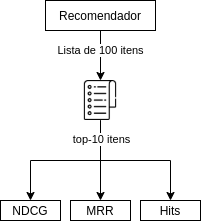
\includegraphics[width=0.25\textwidth]{./imgs/top100-to-top10.png}
    \caption{Avaliação da lista de itens recomendados.}
    \label{fig:aval}
\end{figure}

Também, para a seleção dos melhores hiper-parâmetros dos métodos foi feito uma busca de parâmetros com eles utilizando uma execução sobre o treino, sendo separado em outro treino e a validação a partir do \textit{leave-one-out} e o conjunto de hiper-parâmetros da execução com o maior MRR foi selecionado.

Também diversas proposta de recomendadores existem para sistemas tradicionais, ou seja, são soluções gerais que podem ser aplicadas a qualquer dominio. Os seguintes métodos serão utilizados como linhas de base para avaliação:

\begin{enumerate}
  \item Random: modelo simples, para definir o lower bound do problema, que recomenda itens de maneira aleátoria.
  \item Popular: modelo tradicional de baseline de sistemas de recomendação, esse método irá rankear os itens conforme o mais popular. A popularidade foi definida nesse trabalho como o número de diferentes usuários que clicaram no item.
  \item SVD (Singular Value Decomposition): o SVD é um método de fatorização de matrizes que é utilizado em sistemas de recomendação para filtragem colaborativa. 
  \item SVD++: é um método que minimiza uma função objetivo, que inclui um viés geral e outros 2 para os usuários e os itens, utilizando Stochastic Gradient Descent (SGD) assim como regularização com L2.
  \item BilinearNet: é um baseline simples de aprendizado de embeddings com redes neurais, que não usa nenhuma camada e aprende as representações dos usuários e itens.
  \item NeuMF \cite{he2017neural}: é um método baseado em redes neurais, que funde a fatorização generalizada de matrizes por meio de redes neurais com camadas de multilayer perceptron. Uma ilustração do modelo é apresentada abaixo:
  \item LightGCN \cite{he2020lightgcn}: método que aprende os embeddings do usuário e do item propagando-os linearmente no gráfico de interação do usuário com o item e usa a soma ponderada dos embeddings aprendidos em todas as camadas como o embedding final.
\end{enumerate}

\section{Resultados}

Será apresentado uma análise dos resultados nessa seção, começando pela análise das variações da entrada de rede neural e depois avaliando os resultados frente a outras linhas de base competitivas da literatura.



\subsection{Comparação com linhas de base}

A Tabela \ref{tbl:resultsmain} apresenta os resultados dos métodos nas bases de dados descritas anteriormente conforme a política de avaliação também descrita. Primeiramente os resultados indicam que o método proposto ganha significativamente em relação aos outros em todas as bases de dados, indicando a efetividade da combinação de múltiplas informações. Além disso, os métodos tradicionais possuem um acréscimo significativo em relação às métricas quando direcionados a usuários com mais informações, isso demonstra a capacidade dos mesmos de aprenderem sobre as preferências dos usuários, mas também demonstra a incapacidade dos métodos de satisfazerem os usuários em contextos de pouca informação. O método proposto parece inicialmente conseguir ser apto em ambos casos.

Apesar de haver somente um empate, o método proposto apresenta uma superioridade em outras métricas estável o suficiente para consideralo superior as demais linhas de base da literatura. Os outros métodos, de filtragem colaborativa, apresentam maior estabilidade entre as bases $n=5$ e $n=10$ quando na Amazon Clothing, já que a mesma possui mais interações, tornando os métodos de filtragem colaborativa mais fortes, isso já não ocorre na base com menos interações (Amazon Fashion). Os ganhos de de 80\% de MRR, 70\% de NDCG e 108\% de Hits mostram a aptidão da proposta para a recomendação de vestimentas, se mostrando particularmente adequada devido a sua capcidade de composição de múltiplas informações para predição de preferências de usuários.


\begin{table}
\small

\begin{tabular}{llll}
\hline
 Amazon Fashion (n=5)  &                                                        &                                                        &                                                        \\\hline
                       & MRR                                                    & NDCG                                                   & Hits                                                   \\\hline
 Random                & 0.03079                                                & 0.01036                                                & 0.10438                                                \\
 Popular               & 0.24759                                                & 0.04396                                                & 0.32160                                                \\
 SVD                   & 0.23278                                                & 0.03781                                                & 0.27986                                                \\
 SVD++                 & 0.04975                                                & 0.01436                                                & 0.12996                                                \\
 BilinearNet           & 0.23848                                                & 0.03713                                                & 0.27160                                                \\
 NeuMF                 & 0.24200                                                & 0.03942                                                & 0.30068                                                \\
 LightGCN              & 0.25016                                                & 0.03966                                                & 0.28385                                                \\
 MLP*(LightGCN+Popular) & 0.30309\textcolor[rgb]{00,0.45,0.10}{$\blacktriangle$} & 0.06172\textcolor[rgb]{00,0.45,0.10}{$\blacktriangle$} & 0.52578\textcolor[rgb]{00,0.45,0.10}{$\blacktriangle$} \\\hline
 Amazon Fashion (n=10) &                                                        &                                                        &                                                        \\\hline
                       & MRR                                                    & NDCG                                                   & Hits                                                   \\\hline
 Random                & 0.02915                                                & 0.01025                                                & 0.09219                                                \\
 Popular               & 0.06004                                                & 0.01181                                                & 0.09531                                                \\
 SVD                   & 0.07039                                                & 0.01319                                                & 0.11094                                                \\
 SVD++                 & 0.08332                                                & 0.02058                                                & 0.15625                                                \\
 BilinearNet           & 0.06967                                                & 0.01056                                                & 0.07969                                                \\
 NeuMF                 & 0.08320                                                & 0.01513                                                & 0.12187                                                \\
 LightGCN              & 0.06568                                                & 0.01206                                                & 0.09688                                                \\
 MLP*(LightGCN+Popular) & 0.15010\textcolor[rgb]{00,0.45,0.10}{$\blacktriangle$} & 0.03511\textcolor[rgb]{00,0.45,0.10}{$\blacktriangle$} & 0.32500\textcolor[rgb]{00,0.45,0.10}{$\blacktriangle$} \\\hline
 Amazon Clothing (n=5)    &                                                        &                                                        &                                                        \\\hline
                       & MRR                                                    & NDCG                                                   & Hits                                                   \\\hline
 Random                & 0.02976                                                & 0.01016                                                & 0.10181                                                \\
 Popular               & 0.08635                                                & 0.02169                                                & 0.17545                                                \\
 SVD                   & 0.05184                                                & 0.01231                                                & 0.10670                                                \\
 SVD++                 & 0.07245                                                & 0.01915                                                & 0.16400                                                \\
 BilinearNet           & 0.09200                                                & 0.01599                                                & 0.12375                                                \\
 NeuMF                 & 0.09753                                                & 0.01838                                                & 0.14859                                                \\
 LightGCN              & 0.09131                                                & 0.01731                                                & 0.13116                                                \\
 MLP*(LightGCN+Popular) & 0.13566\textcolor[rgb]{00,0.45,0.10}{$\blacktriangle$} & 0.03294\textcolor[rgb]{00,0.45,0.10}{$\blacktriangle$} & 0.26637\textcolor[rgb]{00,0.45,0.10}{$\blacktriangle$} \\\hline
 Amazon Clothing (n=10)   &                                                        &                                                        &                                                        \\\hline
                       & MRR                                                    & NDCG                                                   & Hits                                                   \\\hline
 Random                & 0.03062                                                & 0.01033                                                & 0.10390                                                \\
 Popular               & 0.06673                                                & 0.01475                                                & 0.11803                                                \\
 SVD                   & 0.05201                                                & 0.00990                                                & 0.08327                                                \\
 SVD++                 & 0.08378                                                & 0.02174                                                & 0.18374                                                \\
 BilinearNet           & 0.07173                                                & 0.01186                                                & 0.09247                                                \\
 NeuMF                 & 0.07917                                                & 0.01586                                                & 0.13429                                                \\
 LightGCN              & 0.07110                                                & 0.01282                                                & 0.09684                                                \\
 MLP*(LightGCN+Popular) & 0.10998\textcolor[rgb]{00,0.45,0.10}{$\blacktriangle$} & 0.02353\textcolor[rgb]{00,0.45,0.10}{$\blacktriangle$} & 0.18494\textcolor[rgb]{0.7,0.7,0.0}{$\bullet$}         \\
\hline
\end{tabular}

\caption{\small Desempenho de diferentes métodos em quatro conjuntos de dados. O método de stacking (MLP) alcança melhorias estatisticamente significativas, superando todas as linhas de base. o símbolo \textcolor [rgb]{00,0.45,0.10}{$\blacktriangle$} denota ganhos significativos e \textcolor[rgb]{0.7,0.7,0.0}{$\bullet$} denota empates estátisticos pela aplicação do teste t de Student com um valor $p$ $\bm{=0,05}$ sobre a melhor linha de base.}
\label{tbl:resultsmain}
\end{table}

\subsection{Experimento fatorial}

Nessa subseção será desenvolvido uma espécie de experimento fatorial sobre entradas para o método de stacking proposto. O objetivo principal desse experimento é identificar as explicações para os resultados obtidos atráves do método e quais os maiores fatores de impacto para o resultado final. Nesse experimento as entradas para o método serão:

\begin{enumerate}
  \item Contexto: consiste dos meta-dados dos usuários, itens e interação;
  \item LightGCN: pontuação atribuída pelo LightGCN, dado o par usuário-item;
  \item Popular: pontuação atribuída Popular, dado um item.
\end{enumerate}

Esses dois métodos foram escolhidos, pois, um deles é de filtragem colaborativa e estado-da-arte na literatura que é capaz de modelar representações complexas do comportamento de interação do usuário,  e o outro é um método não-personalizado que se mostra muito efetivo em diversos cenários, sendo robusto em alguns casos que são desafios para métodos de filtragem colaborativa (i.e., cold-start). Nos conjuntos de entrada será considerado que haverá sempre um dos métodos, LightGCN ou Popular.

A Tabela \ref{tbl:resultsfact} mostra os resultados obtidos a partir do experimento fatorial. O primeiro ponto que pode ser visto é que por mais que não sejam todos, existem diversos casos no qual a combinação dos métodos sem inclusão de contexto consegue ser competitivo com as melhores combinações. Porém no geral, os melhores valores das métricas estão atrelados as combinações que incluem meta-dados. Particularmente, temos que o Popular na Amazon Fashion (n=10) e Amazon Cloth (n=10) consegue os maiores valores em algumas métricas, somente com a inclusão de contexto em um método simples foi possível um ganho significativo. Isto demonstra a particularidade da base de por possuir muitos usuários que interagem pouco, possui uma grande tendência a o contexto dizer muito sobre as preferências de um usuário. Somente com a combinação da popularidade com o contexto é possível representar computacionalmente muitos padrões complexos de consumo do usuário.

Alguns métodos também se mostram mais adequados a certas bases de dados, é importante notar que cada uma dessas bases são extremamente caracteristicas devido a seu número de usuários, número de interações e etc.

\begin{table}
\small
\begin{tabular}{llll}
\hline
 Amazon Fashion (n=5)     &                                                         &                                                         &                                                         \\\hline
                          & MRR                                                     & NDCG                                                    & Hits                                                    \\\hline
 MLP*(Popular + LightGCN) & 0.30309                                                 & \textbf{0.06172}                                                 & \textbf{0.52578}                                                 \\
 MLP*(Popular)            & 0.09041                                                 & 0.01810                                                 & 0.17247                                                 \\
 MLP*(LightGCN)           & 0.07032                                                 & 0.01716                                                 & 0.15691                                                 \\
 MLP(Popular)             & 0.24572                                                 & 0.04366                                                 & 0.32179                                                 \\
 MLP(LightGCN)            & 0.05444                                                 & 0.01093                                                 & 0.08317                                                 \\
 MLP(Popular + LightGCN)  & \textbf{0.30633}          & 0.05973 & 0.49368 \\\hline
 Amazon Fashion (n=10)    &                                                         &                                                         &                                                         \\\hline
                          & MRR                                                     & NDCG                                                    & Hits                                                    \\\hline
 MLP*(Popular + LightGCN) & 0.15010                                                 & 0.03511                                                 & 0.32500                                                 \\
 MLP*(Popular)            & \textbf{0.31656}                                                 & \textbf{0.09285}                                                 & 0.77656                                                 \\
 MLP*(LightGCN)           & 0.06457                                                 & 0.01280                                                 & 0.10156                                                 \\
 MLP(Popular)             & 0.25637                                                 & 0.08096                                                 & 0.72969                                                 \\
 MLP(LightGCN)            & 0.02594                                                 & 0.00547                                                 & 0.05000                                                 \\
 MLP(Popular + LightGCN)  & 0.24800 & 0.08222 & \textbf{0.80625}  \\\hline
 Amazon Cloth (n=5)       &                                                         &                                                         &                                                         \\\hline
                          & MRR                                                     & NDCG                                                    & Hits                                                    \\\hline
 MLP*(Popular + LightGCN) & 0.13566                                                 & 0.03294                                                 & 0.26637                                                 \\
 MLP*(Popular)            & 0.07004                                                 & 0.01872                                                 & 0.14926                                                 \\
 MLP*(LightGCN)           & \textbf{0.19476}                                                 & 0.03778                                                 & 0.28536                                                 \\
 MLP(Popular)             & 0.19086                                                 & \textbf{0.04515}                                                 & \textbf{0.38982}                                                 \\
 MLP(LightGCN)            & 0.10115                                                 & 0.02085                                                 & 0.15444                                                 \\
 MLP(Popular + LightGCN)  & 0.06994 & 0.01887 & 0.14880 \\\hline
 Amazon Cloth (n=10)      &                                                         &                                                         &                                                         \\\hline
                          & MRR                                                     & NDCG                                                    & Hits                                                    \\\hline
 MLP*(Popular + LightGCN) & 0.10998                                                 & 0.02353                                                 & 0.18494                                                 \\
 MLP*(Popular)            & \textbf{0.34585}                                                 & \textbf{0.08145}                                                 & \textbf{0.64870}                                                 \\
 MLP*(LightGCN)           & 0.17003                                                 & 0.02881                                                 & 0.22007                                                 \\
 MLP(Popular)             & 0.33231                                                 & 0.07267                                                 & 0.54610                                                 \\
 MLP(LightGCN)            & 0.04105                                                 & 0.00744                                                 & 0.05604                                                 \\
 MLP(Popular + LightGCN)  & 0.09538 & 0.02007 & 0.15409 \\
\hline
\end{tabular}

\caption{\small Resultados do experimento fatorial da proposta. O asterisco ''*'' indica a utilização de contexto e sua omissão a não utilização. Os maiores valores estão destacados em \textbf{negrito}.}
\label{tbl:resultsfact}
\end{table}


\section{Conclusão}

Foi desenvolvido um método que consegue combinar em contexto de um domínio com métodos de recomendação tradicionais, incorporando essas informações para atingir um nível maior de reconhecimento de padrões de interação para posterior inferência mais precisa das preferências dos usuários. O método é capaz de combinar quaisquer tipos de sistema de recomendação, particulamente neste trabalho combinamos um método de redes neurais de filtragem colaborativa com um método classico não-personalizado. O método apresentado mostrou ganhos significativos de até 80\% de MRR, 70\% de NDCG e 108\% de Hits.

Em trabalhos futuros pretendemos investigar expandir mais as análises, com mais linhas de base assim como mais combinações no \textit{stacking}. Também visamos a aplicação de outras técnicas para dados tabulares que sejam simples e eficiêntes para agregar as informações das pontuações dos sistemas de recomendação com o contexto.


\bibliographystyle{plainnat}
\bibliography{acmart.bib}
\end{document}

\endinput
%%
%% End of file `sample-lualatex.tex'.
